\documentclass[11pt,sigconf]{acmart}

\usepackage{booktabs} % For formal tables

\graphicspath{{figure/}{figures/}}

% Copyright
%\setcopyright{none}
%\setcopyright{acmcopyright}
%\setcopyright{acmlicensed}
\setcopyright{rightsretained}
%\setcopyright{usgov}
%\setcopyright{usgovmixed}
%\setcopyright{cagov}
%\setcopyright{cagovmixed}


% DOI
\acmDOI{10.475/123_4}

% ISBN
\acmISBN{123-4567-24-567/08/06}

%Conference
\acmConference[Spring '22]{CSCI 6502 - Big Data Analytics}{March 2022}{Boulder , CO, USA} 
\acmYear{2022}
\copyrightyear{2022}

\acmPrice{15.00}


\begin{document}
\title{Galaxy Morphological Classification with Big Data: An Analysis of Large Spectral and Photometric Datasets}
\titlenote{Produces the permission block, and copyright information}
\subtitle{Extended Abstract}

\author{Son Pham}
\authornote{Note}
\orcid{1234-5678-9012}
\affiliation{%
  \institution{CU Boulder}
  \city{Boulder} 
  \state{CO} 
}
\email{son.pham-2@colorado.edu}


% The default list of authors is too long for headers}
\renewcommand{\shortauthors}{S. Pham}


\begin{abstract}

\end{abstract}

%
% The code below should be generated by the tool at
% http://dl.acm.org/ccs.cfm
% Please copy and paste the code instead of the example below. 
%
\begin{CCSXML}
  <ccs2012>
  <concept>
  <concept_id>10002950.10003714</concept_id>
  <concept_desc>Mathematics of computing~Mathematical analysis</concept_desc>
  <concept_significance>300</concept_significance>
  </concept>
  <concept>
  <concept_id>10002951.10002952</concept_id>
  <concept_desc>Information systems~Data management systems</concept_desc>
  <concept_significance>300</concept_significance>
  </concept>
  <concept>
  <concept_id>10010147.10010257</concept_id>
  <concept_desc>Computing methodologies~Machine learning</concept_desc>
  <concept_significance>300</concept_significance>
  </concept>
  <concept>
  <concept_id>10010147.10010919</concept_id>
  <concept_desc>Computing methodologies~Distributed computing methodologies</concept_desc>
  <concept_significance>300</concept_significance>
  </concept>
  </ccs2012>
\end{CCSXML}

\ccsdesc[300]{Mathematics of computing~Mathematical analysis}
\ccsdesc[300]{Information systems~Data management systems}
\ccsdesc[300]{Computing methodologies~Machine learning}
\ccsdesc[300]{Computing methodologies~Distributed computing methodologies}
\ccsdesc[300]{Applied computing~Astronomy}

% We no longer use \terms command
%\terms{Theory}

\keywords{ACM proceedings}


\maketitle

\section{Introduction}

% Refer to \verb|acmart.pdf| \cite{veytsmanlatex} (\url{https://www.ctan.org/pkg/acmart}, 
% \url{http://www.acm.org/publications/proceedings-template}) for additional examples and instructions.
Big data analytics is transforming the way scientists and astronomers study the universe. 
With each large scale telescope on the ground or in space, dozens of gigabytes of data 
is being generated per day - an amount that will take an increasingly amount of time
to explore and process. For example, the Hubble Space Telescope generates about 120G of 
scientific data every week \cite{tillman}. Sky surveys conducted by telescopes such as
the Sloan Digital Sky Survey (SDSS) produces data releases each year that can be as high as
100's of TBs. SDSS provides a wide range of data types, such as optical spectra,
infrared spectra, and imaging. 
\\
Recent discoveries, such as the presence of over 100 black holes 
in the center of our Milky Way, was realized using data from decades ago generated by
the Chandra satellite. Scientific and technological advancement in combination led the 
way to this capability. With the increase in computational performance, astronomers 
now have the capabilities to explore these large datasets without the need to invest 
in large ground-based optical telescopes or work in a research lab. 
As big data analytics continue to grow, these discoveries will become more common as 
scientists continue to collect and process more of the data that is available. As technological
advancements grow, they will have more readily available tools and platforms for their 
analysis. With the cummilation telescopes and technologies present today, the entire 
electromagnetic spectrum can be observed within a patch of sky of interest. 
\\
SDSS datasets, such provide many different data types, provides the opportunity to
explore galaxies, stars, and quasars too distant to view for amateur astronomers and 
conduct many different types of analysis on them. The analytics of interest to the
authors include the use of optical imaging and spectral data. Legacy imaging generated 
from prior SDSS programs, if used with machine learning classification techniques, 
can provide automatic classification of morphological properties of these galaxies. 
Quatities measured from these images and spectra readings can also provide information
such as magnitudes, redshifts, and object classifications. In particular, redshift can
be a good indicator of galaxy morphology. 
\\
This paper will go over in detail the approach to perform morphological classification of 
galaxies using these available information from various sources. The main source of interest
for the author is SDSS's data, which includes 100's of terabytes of data covering more
than one-third of the entire celestial sphere \cite{SDSS}.


\section{Literature Survey}

\subsection{External Studies}

\subsection{Studies Based on This Dataset}




\section{Datasets}

SDSS Imaging
\begin{table}[]
  \begin{tabular}{ |p{3cm}|p{2.8cm}|p{1.6cm}|  } \hline
   Parameter & Description & Unit  \\ \hline
   Total unique area covered & 14,555  & sq. deg \\ \hline
   Total area of imaging (including overlaps) & 31,637 & sq. deg \\ \hline
   Individual image field size & 1361x2048 (0.0337) & pixels (sq. deg) \\ \hline
   catalog objects & 1,231,051,050 & (-) \\ \hline
   unique detections & 932,891,133 & (-) \\ \hline
   Median PSF FWHM, r-band & 1.3 & arcsec \\ \hline
   Pixel scale & 0.396 & arcsec \\ \hline
  \end{tabular}
  \end{table}

\section{Approach}

\subsection{Data Cleaning and Pre-Processing}


\subsection{Data Integration}


\subsection{Statistical Analysis}
One of the major issues in working with large datasets is that the standard analytical
evaluation of statistical formulas requires an entire batch of data samples to
be stored in memory for computation. Having 100's of thousands of samples can
quickly exceed the memory limit of an average laptop or computer. This is especially
the case when running analysis on embedded systems where memory is a driving constraint
of performance. Stream processing allows a user to run calculations as the data comes in
and releases memory that held samples of data from previous use.

Welford's method for statistical analysis allows the use of stream processing to
compute some statistical parameters \cite{welford}. This method gives accurate estimates of the 
mean and variance without having to store all the data in memory. The standard process for computing
standard deviation is to compute the mean of the data in one pass, then calculate the square
deviation of values from the mean in the second pass. In crude methods of numerically computing
deviation and means, one can compute the same standard deviation in one pass. Equation \ref{eqn_stddev} shows
this method by accumulating the sums of $x_i$ and $x_{i}^{2}$. This subtraction can result in 
loss of accuracy if the square of the mean is large while the variance is small.

\begin{equation} \label{eqn_stddev}
  \begin{split}
    \sigma =\sqrt{(n\sum_{1\leq i\leq n}x_{i}^{2}-(\sum_{1\leq i\leq n} x_{i})^2)/n(n-1)}
  \end{split}
\end{equation}

Welford's method simply keeps a running sum of the data, number of samples, 
and deviation from data collected so far, and the user can view the sample variance and
mean at anytime during the computational process to view their progression. Equation \ref{eqn_w1} show
the recurrence formula from Welford which takes into account only the current and previous sample values.
Equation \ref{eqn_w2} shows the computation of the mean, and Equation \ref{eqn_w3} for the standard deviation. 

\begin{equation} \label{eqn_w1}
  \begin{split}
    M_{2,n}=M_{2,n-1}+(x_n -\bar{x}_{n-1})(x_n -\bar{x}_{n})
  \end{split}
\end{equation}

\begin{equation} \label{eqn_w2}
  \begin{split}
    \sigma_{n}^{2}=\frac{M_{2,n}}{n}
  \end{split}
\end{equation}

\begin{equation} \label{eqn_w3}
  \begin{split}
    s_{n}^{2}=\frac{M_{2,n}}{n-1}
  \end{split}
\end{equation}






\subsection{Imaging}


\subsection{Spectroscopy}



\begin{figure}[htbp]
  \centering
  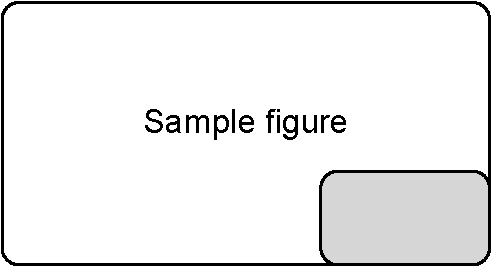
\includegraphics[scale=0.5]{sample-figure}
  \caption{Sample figure}
  \label{fig:sample}
\end{figure}




\section{Evaluation}

 
\subsection{Statistical Analysis}


\subsection{Imaging}


\subsection{Spectroscopy}


\section{Results}





\section{Applications}




\section{Conclusion}





\bibliographystyle{acm}
\bibliography{sigproc} 

\end{document}
